\section{MOS-RMBench-Data}
To systematically evaluate reward models for speech quality assessment, we construct MOS-RMBench, a large-scale benchmark centered on Mean Opinion Score (MOS) and preference supervision. MOS-RMBench integrates diverse MOS datasets into a consistent format based on preferences, addresses inconsistencies in scoring standards by using preference pairs rather than absolute MOS scores, and covers diverse speech scenarios. This chapter introduces the benchmark in three aspects: data sources, the annotation strategy for preference data, and overall dataset statistics.

\subsection{Dataset Source}
MOS-RMBench is constructed based on several widely used speech quality datasets. Specifically, we select BVCC \citep{bvcc}, NISQA \citep{nisqa}, SingMOS \citep{singmos}, SOMOS \citep{somos}, and TMHINT-QI \citep{tmhint-qi} as the primary sources for training and in-domain evaluation. To further assess the cross-domain generalization of models, we incorporate the VMC'23 \cite{vmc23} dataset as an OOD evaluation benchmark. A brief description of each dataset is provided below:

\textbf{BVCC:} The BVCC dataset originates from large-scale listening tests and comprises 7,106 samples, including natural speech and synthetic speech generated by 187 systems spanning diverse TTS and voice conversion (VC) methods. The data sources include Blizzard Challenge, Voice Conversion Challenge, and publicly available samples from ESPnet-TTS \citep{hayashi2020espnet}.

\textbf{NISQA:} NISQA is designed for speech quality assessment in communication networks, covering both simulated distortions and real call recordings. The training and validation sets comprise 11,020 and 2,700 samples, respectively, and consist of simulated and live subsets. The test set contains four subsets, with a total of 952 samples.

\textbf{SingMOS:} SingMOS is an open-source, high-quality singing voice MOS dataset in Chinese and Japanese, containing 3,421 segments from both natural singing and 33 systems. It covers various synthesis techniques including singing voice synthesis (SVS), singing voice conversion (SVC), and vocoder-based re-synthesis.

\textbf{SOMOS:} SOMOS is a large-scale MOS dataset focusing on neural TTS. It contains 20,100 samples synthesized from LJ Speech \citep{ito2017lj} by 200 neural TTS systems and natural speech, all generated using the same LPCNet vocoder \citep{valin2019lpcnet} to isolate acoustic-model differences. MOS-RMBench adopts the SOMOS-clean subset to ensure annotation consistency and reliability.

\textbf{TMHINT-QI:} TMHINT-QI is a MOS dataset focused on Mandarin speech, mainly for evaluating speech enhancement (SE) systems. It contains 24,408 samples generated by adding four types of noise (babble, street, pink, white) at four SNR levels (-2, 0, 2, 5 dB) to clean speech, then processed by five SE systems.

\textbf{VMC'23:} The VMC'23 dataset originates from The VoiceMOS Challenge 2023 \citep{vmc23}. It includes three tracks: (1) French TTS, based on Blizzard Challenge 2023 \citep{perrotin2023blizzard} listening tests, with 1,460 samples; (2) singing voice conversion, based on the Voice Conversion Challenge 2023 \citep{huang2023singing}, containing 4,040 samples; (3) noisy and enhanced speech, based on TMHINT-QI(S) \citep{zezario2024study}, consisting of 1,960 samples.

\subsection{Preference Annotation}
Given the differences in MOS scoring standards across existing datasets, we adopt a preference-based annotation strategy that transforms MOS scores into a unified supervision signal to achieve consistent evaluation. The core idea is to replace absolute MOS scores with relative preferences between paired samples, because absolute scores are susceptible to dataset-specific biases and inconsistent scoring scales. By formulating the task as preference comparison, MOS-RMBench provides a consistent signal across datasets with diverse sources and evaluation standards, enabling fair and robust benchmarking of reward models for speech quality assessment across domains and scenarios.

We first convert all samples into a unified 16 kHz WAV format to ensure consistency in subsequent processing. Following this, we filter out samples with unreliable annotations and partition the remaining data from each source dataset into three categories: (i) samples that share the same speech content but differ in speaker, synthesis system, or speech processing conditions, for example a TTS system or noise perturbation; (ii) samples that share the same speaker or are generated by the same system but differ in speech content; and (iii) samples that differ in both content and speaker or system. To ensure that comparisons are meaningful and consistent, we construct preference pairs within each dataset based on the intrinsic relationships between samples. Specifically, for the first two categories, we group samples by shared content or by shared speaker or system, respectively, then construct preference pairs within each group and ensure that the two samples in each pair have different MOS scores. The sample with the higher MOS is labeled ``chosen", and the one with the lower score is labeled ``rejected". For the third category, since explicit grouping is not feasible, we construct preference pairs directly within the dataset and apply the same ``chosen-rejected" labeling rule. 
Finally, we ensure that the number of constructed preference pairs is balanced across datasets so that subsequent evaluations are not biased toward any particular source.

This annotation strategy yields two primary benefits. First, it ensures that pairwise comparisons reflect meaningful contrasts—either differences in system quality under conditions where the content is matched, or differences in content under conditions where the system is matched. 
Second, by converting absolute MOS values into relative preferences, the strategy reduces sensitivity to dataset-specific scoring standards and annotation biases, which facilitates the integration of heterogeneous MOS sources into a single benchmarking framework.


\subsection{Dataset Statistics}
\textbf{Overview.}
MOS-RMBench constructs a large-scale and balanced preference dataset comprising 55,333 training samples, 9,905 development samples, and 6,240 in-domain test samples from five source datasets, together with 3,000 OOD test samples from the VMC'23 challenge for assessing cross-domain generalization, as summarized in Table~\ref{tab:data-overview}.
The benchmark covers a broad spectrum of speech scenarios, including natural and synthetic speech, singing voice, VC, SVC, SE, and speech with real or simulated noise and distortions, spanning six languages: English, Chinese, Taiwanese Mandarin, Japanese, French, and German.
This diversity in acoustic conditions and linguistic coverage establishes a rigorous foundation for the development and evaluation of reward models, enabling them to achieve more robust perceptual discrimination and to generalize effectively across domains and languages.

\begin{table}[t]
\centering
% \setlength{\abovecaptionskip}{0.2cm} % 调整间距
\setlength{\belowcaptionskip}{0.2cm}

\caption{Statistics of MOS-RMBench across datasets.}
\renewcommand{\arraystretch}{1.1} % 行距
\resizebox{\textwidth}{!}{
\begin{tabular}{lccccc}
\toprule
\textbf{Dataset} & \textbf{Train} & \textbf{Dev} & \textbf{Test}  & \textbf{Scenario} & \textbf{Language} \\
\midrule
BVCC       & 9,948  & 2,132 & 1,000 & natural speech, TTS, VC & English \\
NISQA      & 11,571 & 2,796 & 2,240 & natural \& distorted speech & English, German \\
SingMOS    & 10,000 & 2,720 & 1,000 & natural speech, SVS, SVC & Chinese, Japanese \\
SOMOS      & 13,814 & 2,257 & 1,000 & natural speech, TTS & English \\
TMHINT-QI  & 10,000 & --    & 1,000 & natural \& noisy speech, SE & Taiwanese Mandarin \\
VMC'23     & --     & --    & 3,000    & natural \& noisy speech, TTS, SVS, SVC, SE & French, English, Taiwanese Mandarin \\
\midrule
Overall    & 55,333 & 9,905 & 9,240 & -- & -- \\
\bottomrule
\end{tabular}
}
\label{tab:data-overview}
\end{table}


\begin{figure}[t]
  \centering
  \begin{subfigure}[b]{0.32\textwidth}
    \centering
    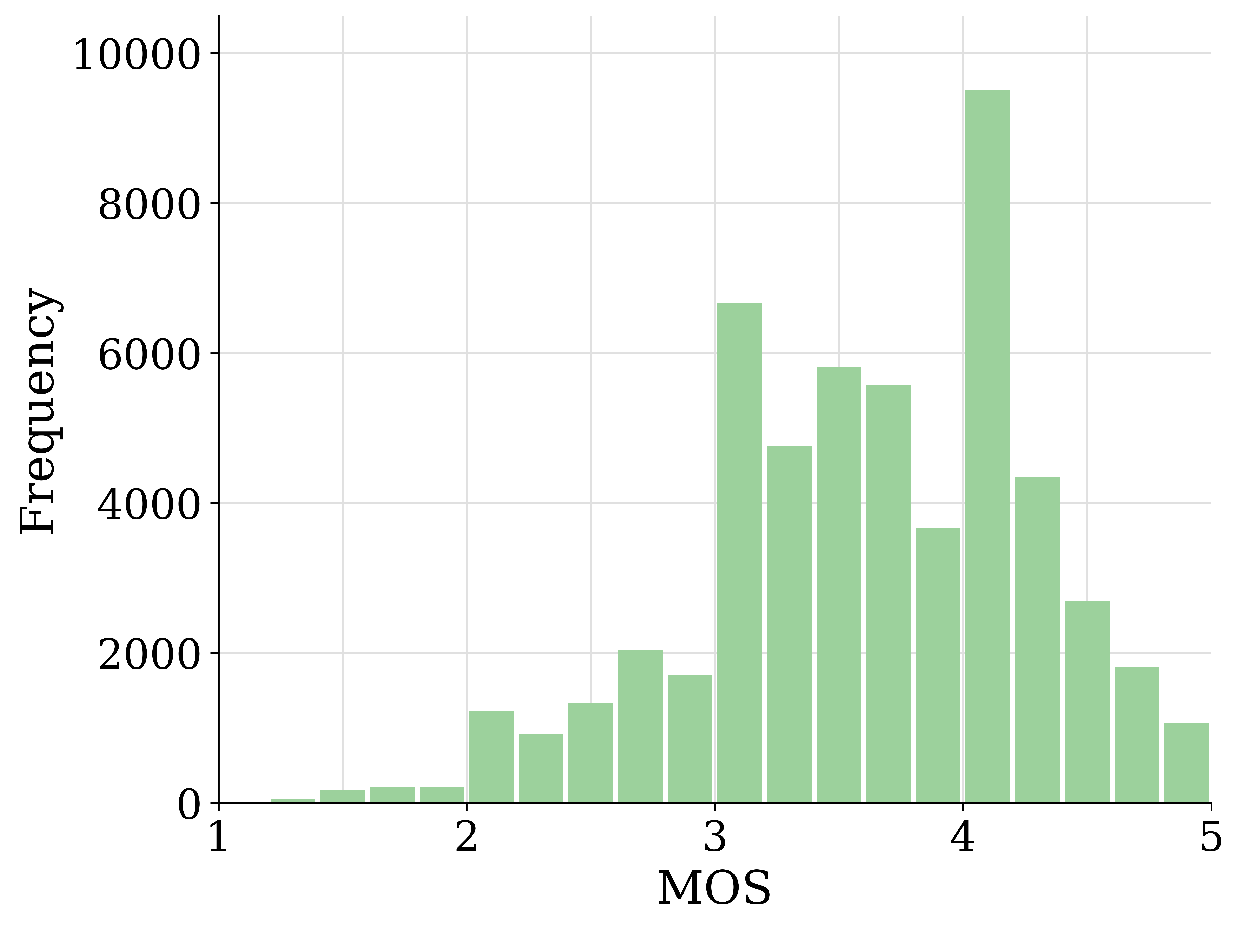
\includegraphics[width=\linewidth]{pictures/chosen_mos_distribution.pdf}
    \caption{Distribution of chosen samples}
  \end{subfigure}
  \begin{subfigure}[b]{0.32\textwidth}
    \centering
    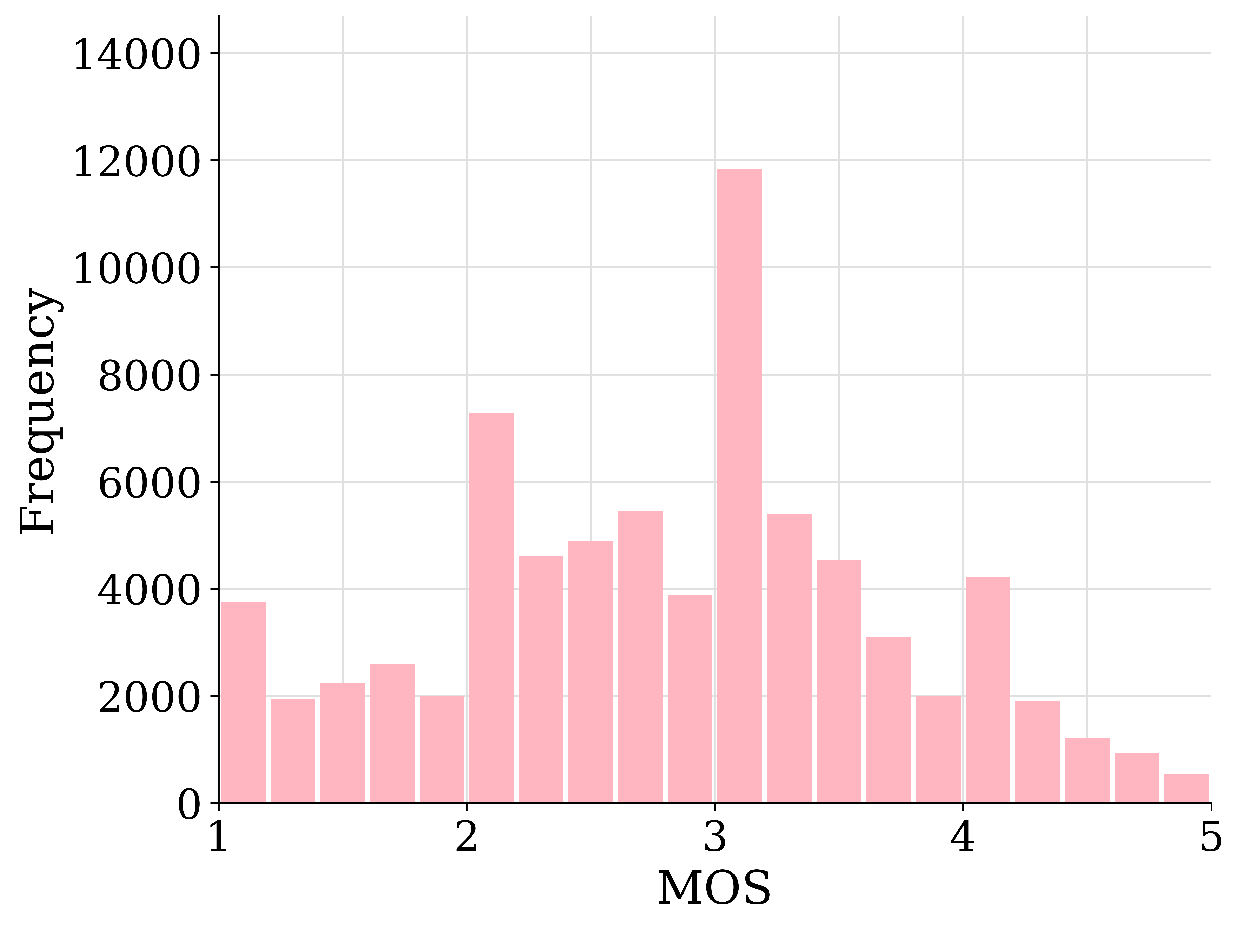
\includegraphics[width=\linewidth]{pictures/rejected_mos_distribution.pdf}
    \caption{Distribution of rejected samples}
  \end{subfigure}
  \begin{subfigure}[b]{0.32\textwidth}
    \centering
    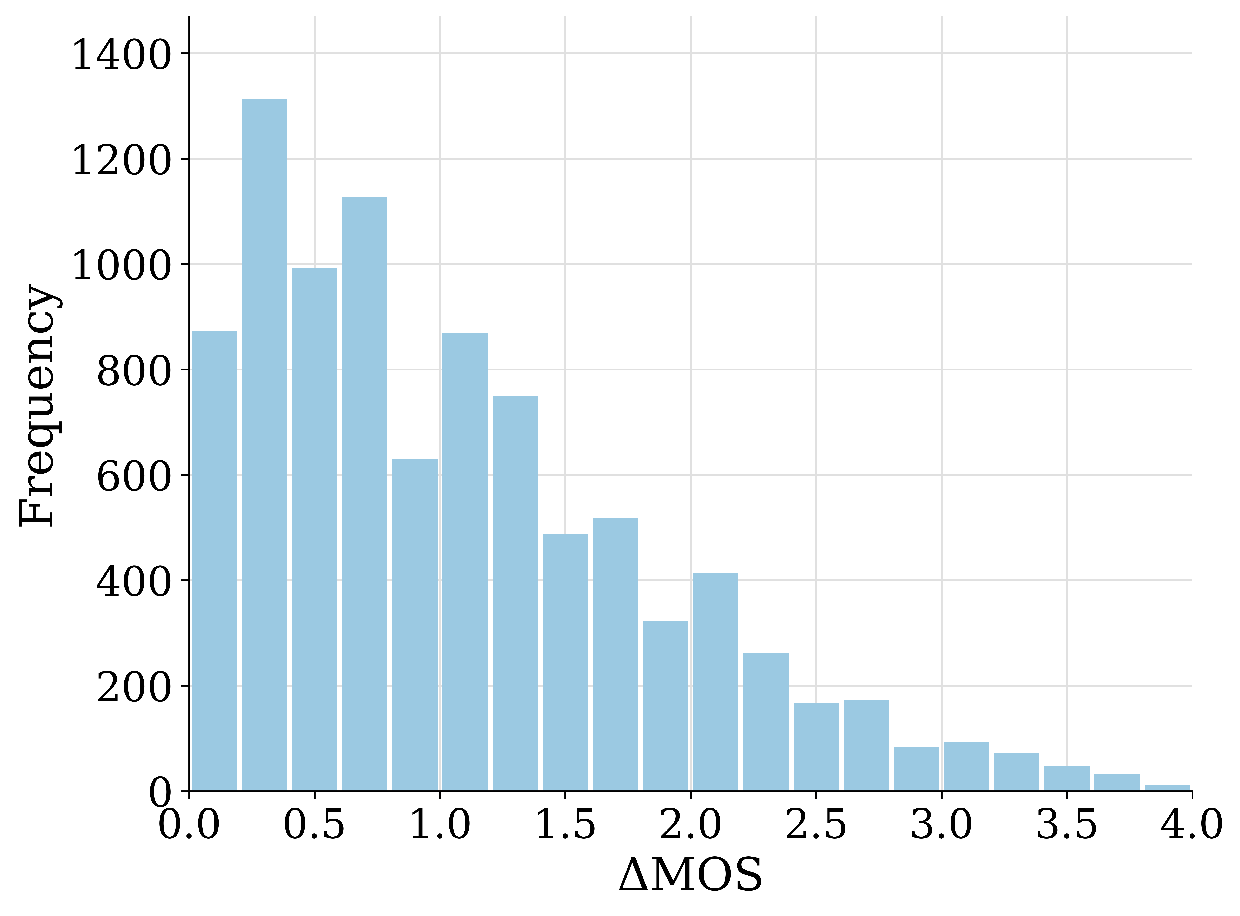
\includegraphics[width=\linewidth]{pictures/delta_mos_distribution.pdf}
    \caption{Distribution of $\Delta MOS$}
  \end{subfigure}
  \caption{Distribution of MOS scores in MOS-RMBench. Figures (a) and (b) show the MOS distributions of chosen and rejected samples. Figure (c) presents the distribution of $\Delta MOS$ in the test set.
}
  \label{fig:data-distribution}
\vskip -0.05in
\end{figure}


\textbf{MOS Distribution.}
Figure~\ref{fig:data-distribution} illustrates the distribution of MOS scores within MOS-RMBench. Overall, the MOS ratings of the chosen samples are predominantly concentrated in the range of 3 and above, whereas the rejected samples are largely distributed below 3.5. This clear separation between the two categories reflects the internal consistency and reliability of the preference annotations.
For the test set, the MOS difference ($\Delta MOS$) between each paired sample is mostly within 1.5 points, indicating that a substantial portion of the speech pairs exhibit very similar perceptual quality, which makes the benchmark particularly challenging for speech quality assessment.

